\documentclass{article}
\usepackage{amsfonts, amssymb, amsmath}
\usepackage{amsthm, thmtools}
\usepackage{framed}
\usepackage{fullpage}
\usepackage{autobreak}
\usepackage{enumerate}
\usepackage{xcolor}
\usepackage{bbm}
\usepackage{hyperref}
\usepackage{graphicx}
\usepackage{float}
\usepackage{geometry}
\geometry{
left=1in,
top=1in,
right=1in,
bottom=1in,
}
\usepackage[skip=1em]{parskip}
\usepackage{setspace}
\setstretch{1.25}
\allowdisplaybreaks
\setlength\parindent{0pt}

\title{\vspace{-1cm}Useful results from measure theory, real analysis and beyond}
\author{Jess Kunke}
\date{Summer 2023}

\begin{document}

\maketitle

\section*{Fundamentals of logic and related proof methods}

The logical statement ``If A, then B" can also be written ``A implies B" or ``All A are B". For example, if a shape is a square, then it is a rectangle. Square implies rectangle. All squares are rectangles.

Any logical statement ``If A, then B" has three related statements: the converse, the contrapositive, and the inverse.

The \textbf{converse} of a logical statement such as ``If A, then B" is ``If B, then A". A statement and its converse are not generally equivalent; an if and only if statement ``A iff B" is when the statement and its converse are equivalent (they are always either both true or both false). Example: a square is a rectangle, but not all rectangles are squares. So if A is ``this shape is a square" and B is ``this shape is a rectangle", the statement ``if A, then B" is true, but its converse is not.

The \textbf{contrapositive} of a logical statement such as ``If A, then B" is ``If not B, then not A". The contrapositive of a statement is true if and only if the original statement is true; they are equivalent. For example, suppose the front door is the only entrance/exit to my apartment. If I leave my apartment (A), I must have opened the front door (B).  Equivalently, if I haven't opened the front door (not B), then I can't have left my apartment (not A). You can prove a statement by proving its contrapositive; this is called \textbf{proof by contraposition}.

The \textbf{inverse} of a logical statement such as ``If A, then B" is ``If not A, then not B". The inverse is the contrapositive of the converse (convince yourself by looking at the above definitions); therefore it is logically equivalent to the converse of the original statement, but not generally to the original statement itself. This is a common logical error, thinking that a statement being true implies that its inverse is true.

Additionally, the \textbf{negation} of a logical statement such as ``If A, then B" is not a new statement; rather, it refers to flipping the truth value of the statement. So if ``If A, then B" is true, its negation is ``It is not true that if A, then B," or ``A does not necessarily imply B". Similarly, if the original statement is false, the negation is ``the original statement is true". You can prove a statement is true by proving that its negation is false; this is called \textbf{proof by contradiction}.

\textbf{Proof by induction} is another important proof method for cases in which you wish to show that a statement applies for all $n = 1, 2, ...$ or some other countably infinite index. The proof is done in two steps. First you prove that the statement holds for $n=1$. Second, you prove that \textit{if} the statement holds for $n-1$, then it holds for $n$. Together, these two steps demonstrate that the statement holds for all $n$.



\section*{Set theory}

\large \textbf{Distributive law:}

\large \textbf{de Morgan's laws:} The complement of the intersection (or union) is the union (or intersection) of the complements. In other words, for an arbitrary (not necessarily countable) collection of sets $\{A_i\}_{i\in I}$ for some index set $I$, \[\left(\cap_i A_i\right)^\mathsf{c} = \cup_i \left(A_i^\mathsf{c}\right), \quad \left(\cup_i A_i\right)^\mathsf{c} = \cap_i \left(A_i^\mathsf{c}\right).\]

\large \textbf{Other key vocabulary and examples:}

\begin{itemize}
    \item Set relations, equivalence relations, equivalence classes
    \item Functions
    \begin{itemize}
        \item Domain, range, codomain. Remember: functions always map the entire domain but may not map to the entire range. The subset of the range to which a function maps the entire domain is called the codomain. For instance, one might say $f: \mathbb{R} \to \mathbb{R}$ defined by $f(x) = x^2$; in this case, $\mathbb{R}$ is the domain, $\mathbb{R}$ is the range, and the set of nonnegative real numbers is the co-domain.
        \item One-to-one/injection, onto/surjection, and bijection/invertible (one-to-one and onto); see Figure \ref{fig:bijection}.
    \end{itemize}
    \item Image and preimage
    \item Rational and irrational numbers, integers
    \item Dirichlet function
    \item Empty set
    \item Cardinality: we say two sets have the same cardinality if there is a bijection between them
    \item Finite, countable (same cardinality as the natural or counting numbers), uncountable
    \item Dedekind theorem: a set $A$ is infinite if and only if there is a subset $S\subset A$ that has the same cardinality as $A$.
    \item The power set of a set $A$, often denoted by $2^A$, is the set of all subsets of $A$.  For example, if $A = \{0, 1\}$, the set containing the two numbers 0 and 1, then $2^A = \{\emptyset, \{0\}, \{1\}, A\}$.
    \item Cantor's theorem: the cardinality of $2^A$ is always bigger than the cardinality of $A$.
    \item Least upper bound, also called supremum. If the supremum exists, it is unique. Sometimes the maximum of a set does not exist but its upper bound does; for example, there is no largest number in the set (0,1) because you can get arbitrarily close to 1, but 1 is the supremum of the set.
    \item Binomial theorem
    \item Between any two rational numbers is an irrational number, and between any two irrational numbers is a rational number.
\end{itemize}

\begin{figure}
    \centering
    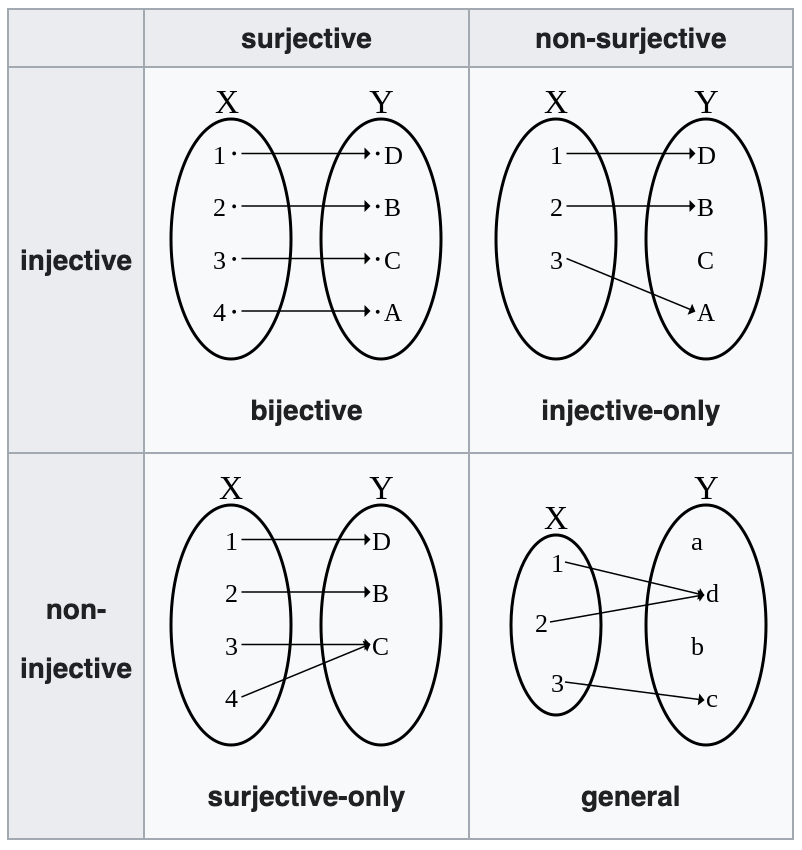
\includegraphics[width=0.5\textwidth]{figures/injection-surjection-bijection.png}
    \caption{Injections, surjections, and bijections. From wikipedia.}
    \label{fig:bijection}
\end{figure}

\section*{Real analysis}

\subsection*{Sequences and convergence}

If a sequence converges, then it is bounded and the limit is unique.

Monotonic can mean strictly increasing, strictly decreasing, nonincreasing, or nondecreasing.

If a monotone increasing sequence is bounded above, then it must converge. If a monotone decreasing sequence is bounded below, then it must converge.

\large \textbf{The sandwich/squeeze/pinching theorem:} Suppose two sequences $\{a_i\}$ and $\{b_i\}$ converge to the same limit, and a third sequence $\{b_i\}$ satifies $a_i \le b_i \le c_i$ for all $i$. Then $\{b_i\}$ also converges, and its limit is the same as the other two sequences.

Definition: A sequence $\{a_i\}$ is a \textbf{Cauchy sequence} if for each $\epsilon > 0$ there is an integer $N > 0$ such that $|a_j-a_k| < \epsilon$ for any $j,k > N$. Properties: Cauchy sequences are bounded, and a sequence of real numbers is Cauchy if and only if it is convergent.

\large \textbf{Bolzano-Weierstrass theorem:} As long as a (not necessarily convergent) sequence $\{a_n\}_{n\ge 1}$ of real numbers is bounded, there exists a subsequence $\{a_{n_k}\}_{k\ge 1}$ of that sequence that converges to some value.

lim sup and lim inf always exist

Common sequences and their convergence: https://mathcs.org/analysis/reals/numseq/speseq.html

Convergence tests for series: https://mathcs.org/analysis/reals/numser/tests.html

Common series: https://mathcs.org/analysis/reals/numser/speserie.html

\subsubsection*{Set topology}

A subset $S$ of $\mathbb{R}$ is called \textbf{open} if for each $x \in S$ there exists an $\epsilon > 0$ such that the interval $(x-\epsilon, x+\epsilon) \subseteq S$. This interval is often called a neighborhood or $\epsilon$-neighborhood of $x$. A set is closed if its complement is open.

Compact sets, perfect sets

Example: the Cantor set is closed, compact, and perfect. 

Dense sets?

\subsection*{Functions}

Epsilon-delta definition of the limit of a function

Definition of continuity

Removable, jump, and essential discontinuities

Max-Min theorem

Intermediate Value Theorem

Mean Value Theorem

Uniform versus pointwise convergence: https://mathcs.org/analysis/reals/funseq/uconv.html

Weierstrass Convergence Theorem

Taylor's theorem with the explicit Lagrange remainder term





\end{document}
